\section{Literature Review}
\label{ch:literaturereview}


% \begin{figure}
%     \centering
%     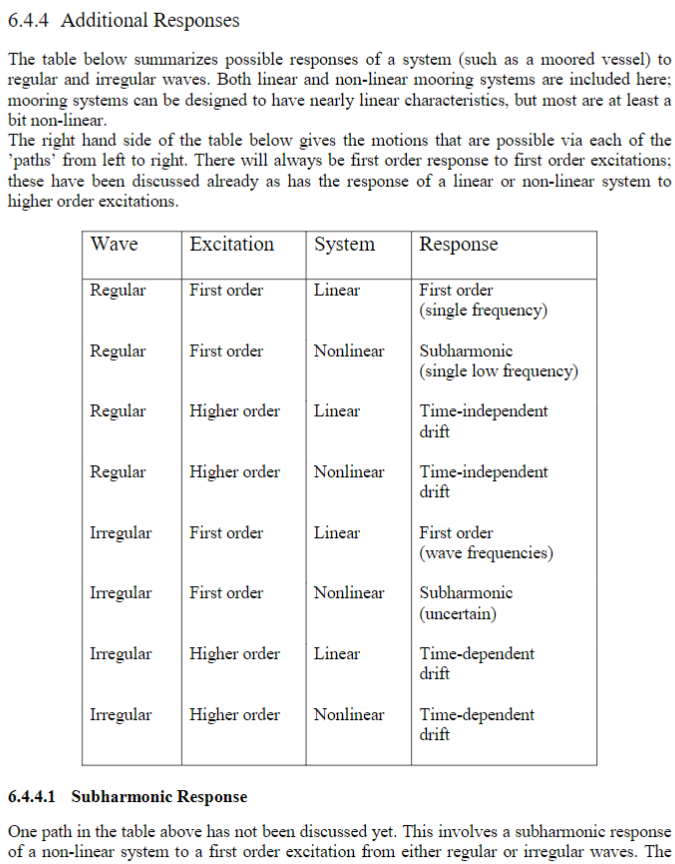
\includegraphics[width=\linewidth]{figures/Literature_Introduction/to_discuss_book_offshorehydromechanics.PNG}
%     \caption{Caption}
%     \label{fig:my_label}
% \end{figure}

% \begin{figure}
%     \centering
%     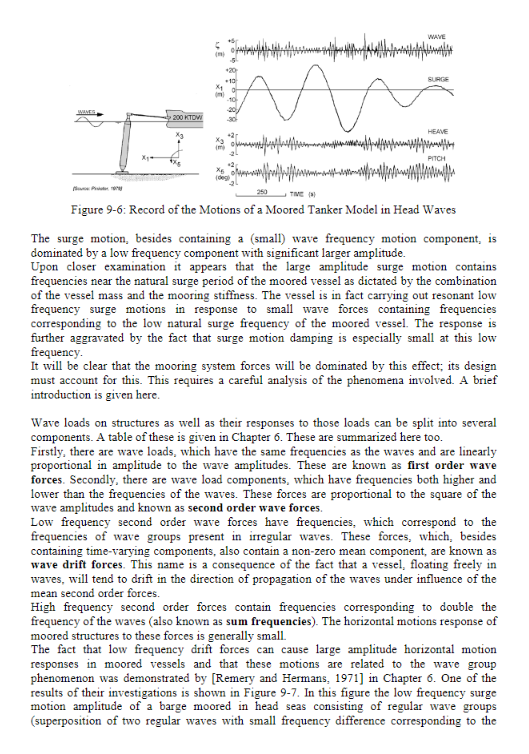
\includegraphics[width=\linewidth]{figures/Literature_Introduction/to_discuss2_book_offshorehydromechanics.PNG}
%     \caption{Caption}
%     \label{fig:largeexcitation_lowfreq}
% \end{figure}


\label{ch: background and literature}


%%%%%%%%%%%%%%%%%%%%%%%%%%%%%%%%%%%%%%%%%%%%%%%%%%%%%%%%%%%%%%%%%%%%%%%%%%
\section{Studies of floating islands}
\label{sec: floating islands}
%%%%%%%%%%%%%%%%%%%%%%%%%%%%%%%%%%%%%%%%%%%%%%%%%%%%%%%%%%%%%%%%%%%%%%%%%%

% \citep{Waals2018}:\\
% Model tests are done for a floating mega island in large waves up to 15.5 m Hs. Motions are studied. Also numerical calculations are done, but without the connections between the modules. Large mooring forces are found at the natural surge frezuency of the modules. In the third wave, there is a response peak at approximately two times the frequency of wave peak period. This third response is not fully understood. Sum frequent second order drift forces might be an explanation. Differences between the numerical model and experimental model tests were large.\\
% \\

% \citep{Otto2019}:\\
% Positive drift forces are found for single triangular body. This means the body will drift towards the waves. This is due to the potential solver which takes no radiation damping and viscous damping into account. \\
% \\
% At the frequencies with the largest motion response, the wave excitation at the leeward modules is close to zero as the waveward islands diffract the incoming wave. \\
% At slightly lower frequencies there is however motion response of the leeward islands, despite that there is no wave excitation acting on them. They are responding to the radiated waves of the waveward triangles.  \\
% For the higher frequencies the interference patterns result in wave excitation on both the waveward and leeward triangles. The motion response on this excitation is however small due to the inertia of the triangles.\\

% \citep{Isope2019}:\\
% In \citep{Isope2019}, design  optimisations  have  been performed by  varying  the draught, size and shape of the islands, making use of the numerical procedure as described in Otto (2019).


Floating mega-islands can provide an attractive solution for creating more space in coastal areas with the high demand for real estate and the probability that less land will be available in the future due to the rising sea level. They can also serve as a central point where large merchant vessels can unload their cargo without manoeuvring into an inland harbour \citep{businessCase_S@S_D1.1}.\\
\\
Experimental and numerical tests have been performed to study the wave-induced motions of a floating island. A piecewise flexible island has been model tested at MARIN as described in \citet{Waals2018}, where the motion behaviour was investigated under the action of waves. Furthermore, the mooring loads and connector loads were analysed in mild and severe sea states. In \citep{Otto2019}, experimental results and numerical simulations have been compared to describe the behaviour of motion. In \citep{Isope2019}, the same numerical method was used to make design optimisations by varying the draught, size and shape of the islands. The latter three studies selected triangular-shaped modules to restrict the least degrees of freedom of motion possible for each floater \citep{Waals2018}. A project partly funded by the European Union called Space@Sea also conducted an extensive case study on the feasibility of multi-use modular floating islands. This case study has been very extensive, covering all fields necessary to realise functioning floating islands in the open sea. For this master thesis, only the results concerning the hydrodynamic performance will be analysed. Space@Sea made the switch from triangular-shaped modules to square shapes from practical points of view. Square modules are cheaper in manufacturing and can be used more efficiently in urban planning \citep{S@SInventoryRegulations}.  \\
\\



The studies mentioned above concluded what the most important hydrodynamic challenges of realising floating islands are:
\begin{enumerate}
    \item Reducing second-order wave drift forces acting on a floating island.
    \item The reduction in the hydroelastic response of a floating island: first-order motions of the modules are unfavourable for the workability/liveability of the floating island, and they result in high connector loads. 
\end{enumerate}


When a floating structure is placed in the sea, it will experience motions as a result of the action of the waves. To avoid large motions, very large structures are desired when these structures need to serve as living and working spaces for people. But large structures experience large drift forces due to second-order wave forces, which will cause low-frequent high-amplitude motions (see Figure \ref{fig: low freq surge motions}). A mooring system, consisting of several lines connected to the sea bottom, will prevent the floating island from floating away (see the Figure below). 
\begin{figure}[H]
    \centering
    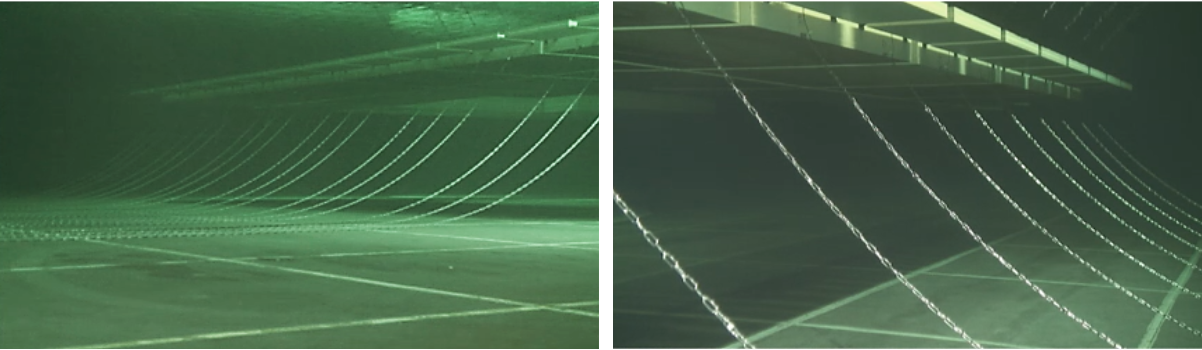
\includegraphics[width=\linewidth]{figures/Literature_Introduction/mooringlines.PNG}
    \caption{Mooring lines of model test \citep{S@S_demonstationatwavetank}}
    \label{fig:mooringlines}
\end{figure}

Due to the catenary effect, a restoring force is created, which allows the structure to drift in these low-frequent and high-amplitude motions, while the weight of the cables will restore the floating island into its mean position. These motions are allowed up to the point that the mooring lines are taut, so the elasticity of the system depends on the amount of slack that can be applied to the lines. When a floating island is placed in deeper water, more slack can be achieved without touching the bottom much. In shallow water, the mooring system needs to be more complex to achieve the same effect. The floating islands' alternative: land reclamation, is less expensive in shallow water as well. In other words, the local water depth is a limiting factor in the feasibility of a floating island. Due to this phenomenon, a conclusion drawn from Space@Sea was that a floating island placed in the Mediterranean Sea is cost-effective, but not in the North Sea \citep{businessCase_S@S_D1.1}. 



However, Space@Sea did not perform extensive research on the possibilities of floating breakwaters. Floating breakwaters can broaden the window of geographical locations in which a functional floating island is possible, by lowering the drift forces acting on the floating island. The processes that take place in these drift forces are elaborated more in appendix \ref{appendix:derivation 2nd order wave force}.\\
\\
 
\begin{figure}
    \centering
    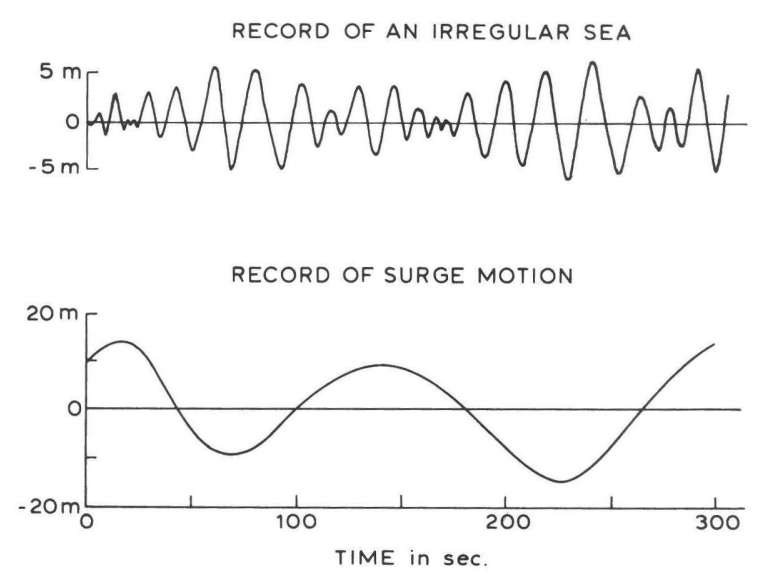
\includegraphics[width=0.7\linewidth]{figures/Literature_Introduction/large_amplitude_low_freq_motions.PNG}
    \caption{Low-frequency surge motions of a moored LNG carrier in irregular head seas \citep{Pinkster1980}}
    \label{fig: low freq surge motions}
\end{figure}



While incident waves at a large floating structure result in wave drift forces, they will also move the structure in higher frequent motions in other degrees of freedom. These motions result in high loads on the connectors of the modules \citep{Isope2019}. This effect is another limiting factor in which a floating island can function until the connector forces are unbearable. Of course, the reduction of both the drift forces and motions goes hand in hand, since attenuating the waves will help against both phenomena. But there is a difference in how attenuation needs to be handled, this is clarified in more detail in Section \ref{sec: floating breakwaters}.

%It should be noted that the relative importance of the drift force increases with increasing wave height as it is quadratic in wave height \citep{Isope2019}. 






% \textbf{todo:} QTF  scales quadratically with the height of the waves! look at Pinkster 1980!, therefore there is a point in which the motions of the island are THE limiting factor OR the drift forces.


%%%%%%%%%%%%%%%%%%%%%%%%%%%%%%%%%%%%%%%%%%%%%%%%%%%%%%%%%%%%%%%%%%%%%%%%%%
\section{Floating breakwaters}
\label{sec: floating breakwaters}
%%%%%%%%%%%%%%%%%%%%%%%%%%%%%%%%%%%%%%%%%%%%%%%%%%%%%%%%%%%%%%%%%%%%%%%%%%

Floating breakwaters have been investigated for a long time. More than 60 configurations of floating breakwaters were recognized by \citep{jones1971transportable} and \citep{richey1974floating}. Later, \citep{Hales1981} separated them into 11 different categories based on their fundamental characteristics. \citep{McCartney1985} chose to subdivide them into four general categories: box, pontoon, mat, and tethered float, and reviewed them based on their performance in reducing wave height and evaluated their construction costs. \citep{Sawaragi1995} classified the floating breakwaters into 3 groups: reflection type, reflection and wave breaking type and friction type. Recently, \citep{Dai2018} did an extensive review on recent research and developments on floating breakwaters, where the different types of floating breakwater were classified into (1) box type, (2) pontoon type, (3) frame type, (4) mat type, (5) tethered float type, (6) horizontal plate type, and (7) other types. However, most of the studies have been done in intermediate to shallow waters (e.g. for the protection of harbours). These floating breakwaters play an important role in providing shelter against wave action by attenuating the energy of incident waves through reflection and/or dissipation. The floating breakwater that was spectacular in terms of its performance is the one in Monaco; it was designed to attenuate 80\% of the wave energy with 2.8 m of significant wave height and 7.2 s of peak period \citep{Ruggeri2017}. The most common is the box-type floating breakwater, which consists of a solid box that floats on the water surface \citep{McCartney1985}. An empirical formula for this kind of breakwater has been formulated by \citep{macagno1953fluid}, where the box is not moving, 2D conditions are assumed, and dissipation is neglected:

\begin{equation}
    K_{\mathrm{t}}=\frac{1}{\sqrt{1+\left[\frac{k W_{\mathrm{f}} \sinh (k h)}{2 \cosh \left(k h-k T_{\mathrm{f}}\right)}\right]^{2}}}
    \label{eq: macagno1953}
\end{equation}
Here, the wave transmission coefficient $K_t$ is expressed as a function of the water depth $h$, the floater width $W_f$, and draught $T_f$.\\
\\

Since conventional bottom-fixed breakwaters can reflect 100\% of incident wave energy, they are most effective in mitigating the hydroelastic response on the floating island. But when the depth of the water increases, its costs will become enormous. A significant reduction could also be obtained by using floating-type breakwaters, provided that the draught of the breakwater and the width to wavelength ratio are sufficiently large \citep{Wang2010}. Floating breakwaters are preferred compared to bottom fixed breakwaters in the conditions where
\begin{enumerate}
    \item the bottom does not support bottom-founded breakwaters
    \item the water depth is too large such that bottom-founded breakwaters are too expensive
    \item the water quality has to be sustained due to minimal interference with water circulation and fish migration.
    \item good aesthetics are desired; floating breakwaters have a low profile and present a minimum intrusion on the horizon, particularly for areas with high tide ranges.
    \item a temporary breakwater is desired. 
\end{enumerate}


The main purpose and, therefore, the main research objective of this thesis is more nuanced than attenuating waves alone. In this research, the best design of a floating breakwater is studied to reduce the drift forces and motions of a floating island connected to its lee side. It is proven that reflecting wave energy can have a reduction in the motions of the floating island but will only result in higher drift forces acting on the floating breakwater. Accordingly, it is more beneficial to dissipate the waves than to reflect them. The derivation of this proof is shown in Appendix \ref{appendix:reflectionversusdrift}.
\\


\subsection{Wave forces on marine structures}
The wave forces acting on marine structures have been extensively studied. \citep{Maruo1960} presented a hydrodynamic theory of the drifting force acting on a circular cylinder, a sphere, and other simple solids on a water wave. It was stated that the two-dimensional case of an infinitely long cylinder floating in regular waves with its axis perpendicular to the wave direction has a mean wave drift force of:
\begin{equation}
    \Bar{F} = \frac{1}{8}\rho g H_i^2
\end{equation}

\citep{longuethiggins1977} derived an expression for the mean wave drift force as a function of the incident, reflected, and transmitted wave height:
\begin{equation}
    \Bar{F} = \frac{1}{16}\rho g (H_i^2 + H_r^2 - H_t^2)(1 + \frac{2kh}{sinh(2kh)})
    \label{eq: longuethiggins force}
\end{equation}
Where incident, reflected and transmitted wave heights are shown as, respectively $H_i$, $H_r$ and $H_t$, the wave number as $k$ and the water depth as $h$.\\
\\
Also, \citep{longuethiggins1977} confirmed that the mean force on submerged bodies is sometimes reduced and even reversed. An explanation is suggested in terms of the "wave setup" produced by breaking waves.\\
\\

Wave loads on structures and their responses can be split into several components, which is discussed extensively in the doctor's thesis of \citep{Pinkster1980} and later summarized in \citep{journee2000offshore}. They are also shown in the following content.
First, wave loads that have the same frequencies as the waves and are linearly proportional to the amplitude of those waves are known as \textbf{first order wave forces}. Second, there are wave force components with a frequency higher than or lower than the wave frequency; they are called \textbf{second order wave forces}. 
Second-order low-frequency wave forces have frequencies, which correspond to the frequencies of wave groups present in irregular waves. These forces contain a time-dependent part, but also have a non-zero mean, which is called \textbf{mean wave drift force}.
The second-order high-frequency wave forces contain frequencies that are twice the frequency of the waves, and they are called \textbf{sum frequencies}. The horizontal response of large moored structures to these forces is generally small. The Table below summarises the possible responses of a system to regular and irregular waves. 

\begin{table}
\centering
\begin{tabular}{|l|l|l|l|} 
\hline
\textbf{Wave}      & \textbf{Excitation}   & \textbf{System}    & \textbf{Response}                            \\ 
\hhline{|====|}
Regular   & First order  & Linear    & First order~(single frequency)      \\ 
\hline
Regular   & First order  & Nonlinear & Subharmonic~(single low frequency)  \\ 
\hline
Regular   & Higher order & Linear    & Time-independent~drift              \\ 
\hline
Regular   & Higher order & Nonlinear & Time-independent~drift              \\ 
\hline
Irregular & First order  & Linear    & First order (wave frequencies)      \\ 
\hline
Irregular & First order  & Nonlinear & Subharmonic (uncertain)             \\ 
\hline
Irregular & Higher order & Linear    & Time-dependent~drift                \\ 
\hline
Irregular & Higher order & Nonlinear & Time-dependent~drift                \\
\hline
\end{tabular}
\caption{Possible responses of a structure under the action of waves \citep{journee2000offshore}}
\end{table} 



% \subsection{Wave breaking}
% \label{sec: literature wave breaking}
% -Iribarren\\
% -splunging, spilling and collapsing dependent on iribarren\\
% -is er al onderzoek gedaan naar hoeveelheid dissipatie van allen (wel meeste reflectie bij grote slope though)?\\





% The amount of studies that have been done in the field of floating breakwaters is tremendous. But with the knowledge gained that the wave attenuation is best obtained from viscous dissipation and the floating breakwater is going to be connected to the floating island, the scope of this study is limited much more.  \\
% \\


% \subsection{Useful literature regarding floating breakwaters}
% Although a lot of studies have been done on the topic of floating breakwaters, the choice in setup causes the number of studies which proved to be useful converges drastically. \\
% \\




%many studies have been done, not everything is useful
%focus on dissipative floating breakwaters
%setup is chosen for the floating breakwater connected to the island, to increase stiffness, because this brings a higher potential to absorb wave energy SOURCE.
%pile supported floating breakwaters may be interesting

% \section{Wave conditions}
% \label{sec: wave conditions}
% % -Irregular waves needed for compliance natural frequency of moored structure --> or take regular waves exactly at natural frequency
% % -eventually conclusion of this section has to be: use regular waves, but choose them wisely (simulation time savings)



% %%%%%%%%%%%%%%%%%%%%%%%%%%%%%%%%%%%%%%%%%%%%%%%%%%%
\section{Optimisation techniques}
% %%%%%%%%%%%%%%%%%%%%%%%%%%%%%%%%%%%%%%%%%%%%%%%%%%%




% % %optimize on motions and drift forces 
% % \textbf{todo:} uitvinden of irregular waves/ regular waves het beste is, afhankelijk van rekentijd van simulatie


On the basis of the literature study on floating breakwaters, a design for the breakwater will be made that best suits its application. The exact dimensions of this breakwater depend on various external parameters, like the geometry of the floating island connected to the lee-side of the breakwater, the water depth, the maximum allowable mooring forces, and the wave conditions. Since many different configurations of these parameters are possible, a smart optimisation method is used to design the breakwater. Several optimisation techniques and tools are already existing; one of these tools is Design Expert, which is based on the method: \acrfull{doe} and is explained in Section \ref{sec: DoE}



% \textbf{Gevonden literatuur:}:
% -Aerodynamic shape optimisation using novel optimizer based on machine learning techniques \citep{Yan2019}.
% CFD and an optimizer are used to come up with new design.
% Within the optimizer, reinforcement learning is applied to extract the optimisation experience from the semi-empirical method DATCOM using deep neural networks. And transfer learning is implemented to reuse the experience as priori knowledge in the CFD-based optimisation by sharing neural network parameters. \\
% \\
% -A machine learning method for the evaluation of hydrodynamic performance of floating breakwaters in waves \citep{}. 2D simulation for the idealisation of FBs in regular and irregular waves. Hydrodynamic performance is assessed by a machine learning method based on Cuckoo Search-Least Square Support Vector Machine model. Output minimal wave height required.\\
% \\
% \acrfull{MOGA} is one of many engineering optimisation techniques, a guided random search method with the possibility to search a diverse set of solutions with more variables that can be optimized at one time. Solutions are illustrated using Pareto fronts. Compared to the conventional method for solving multi-objective problems, \acrshort{MOGA} takes a relatively short computing time .




% \subsection{Topology optimisation}
% Topology optimisation is well-established tool in computational structural engineering \citep{bendsoe2003topology}. In its simplest realisation in structural engineering, a topological optimisation starts with a certain domain entirely filled up by solid material of a certain density. Then the loads are applied, where the stresses are least, material is discarded or the density of the material is lowered. Then the stresses will be calculated again under the same loads and the same process repeats itself until a high-density material is left only in regions that are critical to fulfil the structural task, and in this way the optimal lightweight structural design is met \citep{Othmer2014}. This method came to the field of \acrfull{cfd} in 2003, where \citep{borrvall2003topology} and \citep{moos2004bionic} presented independently a way to optimize ducted flows. With a fixed inlet and outlet, the starting point with a big domain. Then they used some local criterion to determine whether an area was counterproductive with respect to the chosen objective and iteratively removed parts from the domain. Until the optimal duct between the inlet en outlet were reached of a given installation space. Topology optimisation is different from \textit{shape optimisation} and \textit{sizing optimisation}, because the design can attain any shape within the design space, instead of dealing with predefined configurations. \\
% \\
% Topology optimisation for fluid-structure interaction problems have been studied in \citep{}, \citep{}, \citep{} and \citep{}. 





% % % \subsection{Definition Machine Learning}
% % % Building models from data with optimisation and regression


% \subsection{DAKOTA}
% \label{sec: dakota}
% Dakota (Design and Analysis Toolkit for optimisation and Terascale Applications) is going to be the interface between the simulation code ComFLOW and the iterative analysis method. Dakota contains algorithms for optimisation with gradient and non gradient-based methods; uncertainty quantifications with sampling, reliability, and stochastic expansion methods; parameter estimation with nonlinear least squares methods; and sensitivity/variance analysis with design of experiments and parameter study methods. By employing object-oriented design to implement abstractions of the key components required for iterative system analysis, the Dakota toolkit provides a flexible and extensible problem-solving environment for the design and performance analysis of computational models on high-performance computers \citep{DakotaManual2021}. \\
% \\
% Dakota provides several capabilities:
% \begin{itemize}
%     \item \textbf{MOGA} (described in section 6.2.3.1 of \citep{DakotaManual2021})
%     \item \textbf{Pareto-set strategy} (described in section 14.4 of \citep{DakotaManual2021})
%     \item \textbf{Weighting factor approach for multiobjective reduction:} a composite objective function is constructed from a set of individual objective functions using a user-specified set of weighting factors.
% \end{itemize}

% In engineering, a design tool by combining a \acrfull{cfd} solver and DAKOTA is already developed with the design of wind turbine blades \citep{Quan2020}, helicopter rotor blades \citep{Leusink2015}, barriers for windblown sand mitigation \citep{Horvat2020} and squirrel cage fans \citep{Hocine2021}. The drawback of using a \acrfull{GA} is that it requires a high number of evaluations. This is acceptable for industrial applications when using a low time-consuming \acrshort{cfd} solver, but leads to unreasonable high computational costs when a high fidelity \acrshort{cfd} tool is used. 


% % % \textbf{todo:} hoge snelheden leiden tot kleine tijdsstap (motivatie om enkel de FB te modelleren)


\subsection{\acrfull{doe}}
\label{sec: DoE}
Experimentation is used to find the best result or the final design in all kinds of fields. Think, e.g., of construction, biology, education, communication, science, and art. But mostly it is a costly and time-consuming process. When striving for efficiency, is there a way to streamline the work process to get more learning with less experimentation? Here, \acrfull{doe} comes into play. \acrshort{doe} is a systematic and efficient method that allows scientists and engineers to study the relationship between multiple input variables and key output variables. In short, it can optimise the experimentation process by predicting the trend between the change in input variables on the change in the output of the system. \acrshort{doe} is convenient to use:
\begin{itemize}
    \item To determine whether an input variable affects an output variable
    \item To determine whether input variables interact with the output variable
    \item To model the behaviour of the output variables as a function of input variables
    \item To optimize the output variables
\end{itemize}

%The way to implement \acrshort{doe} is as follows. First, the goal of the experiment is determined, from which a response (a result which you can measure well and has influence on the eventual goal) is obtained. Secondly, constant and variable factors are included. The shape and magnitude of the variable factors will affect the response. Next, a model is included which adequately describes the physical situation. Now, all the input is used to generate a design with \acrshort{doe}. 

Different publications that did a \acrshort{doe} optimisation were reviewed by \citet{Weissman2015}, who found that the application of \acrshort{doe} to the development of pharmaceutical processes has increased greatly over the past 11 years. This paper also summarised several steps on how to implement \acrshort{doe} as follows:

\begin{enumerate}
    \item Define the Objective: What problem needs to be resolved? Frequently, the goal is to optimise a design, but sometimes the design conditions are "locked," and the goal is merely to understand the robustness of the existing conditions. In this case, robustness is defined as probing the impact (if any) of small changes in the continuous factors on the outcome.
    
    \item Define Factors/Variables and Their Ranges: The determination of which factors / variables are included in a \acrshort{doe} depends on the resources. More variables will lead to more evaluations. Therefore, it is imperative to prioritise them, using existing knowledge, into groups that are known to be impactful, suspected, possible, and unlikely. Then, assign high and low settings to the factors selected for inclusion in the study, as is the case when using the common two-level factorial design. These settings must be relevant, achievable, and practical. The end product of this exercise is the creation of \textit{design space}.
    
    \item Define the Responses: These are the measurable outcomes of the process. Responses are related to the objectives. 
    
    \item Select the Experimental Design: The choice depends on the objective, the number of factors, and the available resources. The most common are screening designs in which qualitative information about the relevant factors is obtained. These designs also allow the factors to be ranked in the order in which they impact the response. Screening designs are frequently used to filter irrelevant factors to enable focus on the most relevant factors in a second \acrshort{doe} design, also known as optimisation designs. These latter designs require more experiments than screening designs but generate a more comprehensive model of the response surface. 
    
    \item Generate Reaction Worksheet: The input of all the above information into the software will generate a list of configurations to perform.

\end{enumerate}
%more steps are shown in the paper! but this may be complete for me already.

\acrshort{doe} in combination with \acrshort{cfd} is used earlier in optimising the cooling fan performance by \citet{Hagenmaier2002} and in designing an optimal scram jet by \citet{Srinivasa2014}. The use of \acrshort{doe} and \acrshort{cfd} in the study for the optimal breakwater design has not been done before.



% - trial-and-error method and one factor at a time


% \subsection{Multi-fidelity optimisation}
% % %auke van der ploeg vertelde hierover
% % -definitie

% To speed up the optimisation process, the multi-fidelity approach can be used. Here the largest part of the optimisation is carried out by using a coarser grid, from which the results are refined progressively by increasing the resolution of the design domain. In other words, by incorporating low-fidelity data, the feasibility constraints can be modelled accurately using only a small number of high-fidelity evaluations on the feasibility boundary. This has been done for the aerodynamic design of helicopter blades by \citet{Leusink2015} and in wind farm framework optimisation by \citet{multifidelity_windfarm}

% % -voorbeelden van papers die dit gebruiken (https://onlinelibrary.wiley.com/doi/epdf/10.1002/we.1667) (check wikipedia voor meer onderzoeken)



% %%%%%%%%%%%%%%%%%%%%%%%%%%%%%%%%%%%%%%%%%%%%%%%%%%%

\section{\acrfull{cfd}}
In the field of \acrfull{cfd}, often one or a combination of the following equations is being modeled \citep{vanderPlas2017}:
\begin{itemize}
    \item Navier-Stokes equations (viscous flow)
    \item Euler equations (non-viscous flow) 
    \item potential equations (non-viscous, irrotational flow)
\end{itemize}
These three methods are by no means comprehensive. For most applications, \acrfull{DNS} of the Navier-Stokes equations is too expensive. With a \acrshort{DNS}, the entire range of spatial and temporal scales of turbulence is resolved; from the smallest dissipative scales (Kolmogorov microscales) to the integral length scale $L$ of the motions where most of the kinetic energy is located \citep{Westerweel_Turbulence2016}. A so-called turbulence model can be implemented to save computational time. This is a simplification of the Navier-Stokes equation, a mathematical model in which the effects of turbulence are predicted. 
In the particular field of wave modelling, other techniques are used, such as wave theory or the modelling of, for example, the Boussinesq equations \citep{vanderPlas2017}.\\
\\
In the field of \acrshort{cfd}, a commonly encountered field of engineering application involves modelling of wave impact on an offshore structure. If the geometry is not too complicated, it is still possible to use potential theory in combination with empirical formulae with the prediction of impact forces. To obtain flow around very complicated structures, these formulae do not comply with reality, so \acrshort{DNS} is required.

\subsection{ComFLOW}
\label{subsec: comflow literature review}
%  \textcolor{red}{\textbf{todo: include: Low-order not a problem because cells and time steps need to be small anyway, because of large gradients and discontinuities near the free surface}}\\
%  \\
With exactly this field in mind, a \acrshort{cfd} solver is developed: ComFLOW, which describes the motion of an incompressible viscous fluid. Examples of ComFLOW's applications are as follows:
\begin{itemize}
    \item wave impacts
    \item green water loading on ships
    \item liquid sloshing in LNG carriers
\end{itemize}

The solver has its roots in simulating the liquid sloshing on board spacecraft \citep{veldman1984axisymmetric}. For this application, it was developed for microgravity conditions, where surface tension played a dominant role. At Deltares Research Institute, the code was extended to enable simulation of wave impacts. In the 1990s, ComFLOW found its applications in offshore structures, when fully 3D flow around complex geometries could be simulated. Furthermore, the latest developments concentrated on free-surface simulation, wave propagation, wave impact simulation, and the addition of a two-phase flow model \citep{Kleefsman2005}, \citep{Wemmenhove2008}. \\
\\
In this master thesis, the hydrodynamic performance of a floating breakwater is investigated. This performance is expressed by the forces acting on the breakwater and its wave attenuating performance. Due to its interaction with breaking waves, where a two-phase flow model of water and air will occur, ComFLOW is selected as a good fit as the \acrshort{cfd} simulation method. \\
\\
Since dissipation is of great importance in this Master's thesis, it is good to mention how ComFLOW handles wave energy dissipation by wave breaking. In ComFLOW, an energy-preserving turbulence model is implemented, which gives an accurate description of large-scale flow effects. However, small-scale production is controlled by a special treatment of the convection term, instead of adding eddy-viscosity \citep{Luppes2013}. In other words, the physical dissipation in ComFLOW is expected to depend on the size of the grid at the location where wave breaking occurs. \\
\\

ComFLOW has been used before for several applications in the interaction between fluids and structures. A validation of wave run-up calculation methods for a gravity-based structure is done in \citet{Danmeier2008}, sloshing dynamics in LNG tanks was studied by \citet{Wemmenhove2009}, wave-in-deck load on a jacket platform by \citet{Iwanowski2009}, a validation is done by studying ComFLOW performance with wave impacts on a dike by \citet{Wenneker2010}, extreme wave impact on offshore platforms and coastal constructions has been investigated by \citet{Luppes2011}, and recently a shallow water \acrfull{calm} buoy in extreme waves is validated by \citet{Bandringa2021}. 



\section{Scope}
In order to ensure that ComFLOW's results can be used in judging the performance of the breakwaters, it is necessary to study compliance with the reality. Therefore, it is chosen to perform a thorough validation of this \acrshort{cfd} code when waves are interacting with a breakwater. The implementation of this validation in the research questions (see research question 2 in Section \ref{sec: research questions}) shows its prominent role in this thesis. Since wave energy dissipation, reflection and transmission are the most important phenomena to track the performance of breakwaters, these are the parameters were the validation will be based on. \\
\\

% A study to the performance on floating breakwaters with ComFLOW has not been executed before. Therefore, it is chosen to do an extensive validation to this \acrshort{cfd} code when waves are interacting with a breakwater. The implementation of this validation in the research questions (see research question 2 in Section \ref{sec: research questions}) shows its prominent role in this thesis. Since wave energy dissipation, reflection and transmission are the most important phenomena to track the performance of breakwaters, these are the parameters were the validation will be based on. \\
% \\
Increasing the feasibility of floating islands with the help of breakwaters is a new field of research. Therefore, questions need to be answered as: What are the dimensions, shape, and operational water depth of the optimal breakwater in this application for specific wave conditions? A design optimisation, where multiple geometries of breakwaters are going to be evaluated, seems suited well in order to answer these questions. How this is implemented exactly is elaborated more in the following section.
